\documentclass[11pt]{article}

\usepackage[margin=1.5in]{geometry}


\usepackage{lecnotes}
% \usepackage{mpass}
% \lstset{style=verb,language=mpass}
% for this lecture only
\usetikzlibrary{automata,shapes,positioning,matrix,shapes.callouts,decorations.text,patterns,decorations.pathreplacing,matrix,arrows,chains,calc,tikzmark,petri,topaths}
\pgfdeclarelayer{bg}    % declare background layer
\pgfsetlayers{bg,main}
\usepackage{tkz-berge}

\input{lmacros}


\newcommand{\course}{15-316: Software Foundations of Security \& Privacy}
\newcommand{\lecturer}{Matt Fredrikson\footnote{with edits by Giselle Reis, Ryan Riley, and Frank Pfenning}}
\newcommand{\lecdate}{March 31, 2026}
\newcommand{\lecnum}{19}
\newcommand{\lectitle}{Bootstrapping Trust}
\newcommand{\courseurl}{https://15316-cmu.github.io/2026/}

\begin{document}

\maketitle

\section{Introduction}

When we discussed authorization logic, we briefly touched on the topic
of trust. More specifically, authorization logic is distinguished from
other logics that we have looked at by the $A \says P$
construct that represents the fact that principal $A$ affirms
proposition $P$. We saw how to encode decentralized
security policies for systems using $\mb{says}$, so that
various entities can define their own access control rules. The system
components that must ultimately either grant or deny access to
resources can decide which principals to trust, and subsequently
implement a policy by only accepting $\mb{says}$ proclamations
from trusted principals.

We illustrated this using the Grey system~\cite{Bauer05isc}, and now we
will see a different example that emphasizes the importance of
organized trust when making policy decisions. You may be familiar with
the eduroam service, which provides members of participating academic
institutions with wireless network access when they visit another
institution. For example, because both CMU and Pitt are members of
eduroam, when you visit the Pitt campus you can join the wireless SSID
\verb'eduroam', and provide your Andrew ID and password to use the
internet. The same is true at thousands of other institutions across
the world that subscribe to this service.

If you stop to think about it, this is somewhat remarkable given the scale and
disparity in geography and governance among the institutions. How does Pitt know
that you have entered the valid credentials for your Andrew account, which is
managed by CMU? A naive solution might be to distribute the credentials of
all users at eduroam institutions to all of the institutions. Obviously
this will not scale, so perhaps a decentralized authorization policy is called
for.  First of all, the service eduroam can delegate the responsibility of
deciding who is currently a student to the various institutions, for example as
shown below. We use $\mi{er}$ to denote the eduroam principal.
\[
  \begin{array}{l}
    \mi{er} \says \forall x.\, (\mi{cmu} \says \ms{isStudent}(x)) \arrow \ms{isStudent}(x) \\
    \mi{er} \says \forall x.\, (\mi{pitt} \says \ms{isStudent}(x)) \arrow \ms{isStudent}(x)
  \end{array}
\]
Then the main policy governing access to the eduroam wireless network
allows every student to access the network.
\[
  \mi{er} \says \forall x.\, \ms{isStudent}(x) \arrow \ms{canAccess}(x)
\]
The wireless access points responsible for providing the service use this policy
as assumptions $\Gamma$ construct or check a proof of the sequent below when
student $\mi{bob}$ attempts to use the service.
\[
  \Gamma \vdash \mi{er} \says \ms{canAccess}(\mi{bob})
\]
For example, suppose that $\mi{bob}$ attempts to do so.  Rather than writing
out the proof in the sequent calculus, we present it in the form of a proof term.
In the proof-carrying authorization architecture, that is what would be
communicated to the access point.  More conventionally, it provides a
logical justification for granting access but remains implicit in the code
implementing access control for the network.
\[
  \begin{array}{lcl}
    c_1 & : & \mi{er} \says \forall x.\, (\mi{cmu} \says \ms{isStudent}(x)) \arrow \ms{isStudent}(x) \\
    c_2 & : & \mi{er} \says \forall x.\, \ms{isStudent}(x) \arrow \ms{canAccess}(x) \\[1ex]
    c_3 & : & \mi{cmu} \says \ms{isStudent}(\mi{bob}) \\
    \vdash \\
    ?M & : & \mi{er} \says \ms{canAccess}(\mi{bob})
  \end{array}
\]
\begin{tabbing}
  $?M = $ \= $\{\,$ \= \\
  \>\> $\mb{let}\; \{x_1\}_{\mi{er}} = c_1\; \mb{in}$ \\
  \>\> $\mb{let}\; \{x_2\}_{\mi{er}} = c_2\; \mb{in}$ \\
  \>\> $\mb{let}\; x_4 = x_1\; \mi{bob}\; c_3\; \mb{in}$ \\
  \>\> $x_2\; \mi{bob}\; x_4$ \\
  \> $\}_{\mi{er}}$
\end{tabbing}
You may want to refresh your understanding of the details from
the notes to \href{\courseurl/lectures/18-proofrep.pdf}{Lecture 18}.

Because the derivation above will be about the same for any user,
except for the details of institution and user names, the endpoint
need not recompute or check it for each login. Access boils down to a
trusted institution's endorsement that the user is legitimate and
eligible for the service, so instead perhaps users' devices can just
send evidence of the endorsement directly, or the endpoint can obtain
it by some other means.

But how can the access point be sure that this evidence is authentic?
We hinted in the last lecture that digital signatures utilizing
cryptography are a common solution. But the cryptographic techniques
that enable digital signatures require keys, which are either
secrets distributed among trustworthy parties, or public objects that
can be reliably associated with individuals or organizations.

For example, $\mi{cmu}$ could sign and date a certificate stating that
$\mi{bob}$ is currently a student, perhaps with a timeout to account for his
expected graduation date. It would do so using its private key, known
only to CMU, and the access point would verify it by checking the signature
against $\mi{cmu}$'s public key. How does the access point know that it
is using the correct public key? What if someone tricked it into using a
different public key, associated with an attacker's private key, so that it
would trust statements signed by the attacker as coming from $\mi{cmu}$?

We will address this topic today, looking more closely at digital
certificates and Public Key Infrastructure (PKI), which is a
distributed mechanism for managing the trust needed to solve the
problems introduced in this example.

\section{Digital Certificates \& Certificate Authorities}

\newcommand{\sk}[1]{\ensuremath{\mi{sk/#1}}}
\newcommand{\pk}[1]{\ensuremath{\mi{pk/#1}}}

\newcommand{\sign}[1]{\ms{sign}_{#1}}
\newcommand{\verify}[1]{\ms{verify}_{#1}}
\newcommand{\cert}[2]{\ms{cert}_{{#1} \arrow {#2}}}
\newcommand{\enc}[1]{\ms{enc}_{{#1}}}

For the rest of this lecture, we will assume that all principals $A$ have a
secret key \sk{A} and a public key \pk{A}. Suppose in the context of the running
example from the previous section that the eduroam principal generates the
public/private key pairs for all participating institutions.

\paragraph{Digital signatures.}
One of the main applications of public/secret key pairs is to
digital signatures, which we have referenced informally before.
A digital signature scheme consists of three algorithms, for
generating keys, signing messages, and verifying signatures,
respectively. We will always assume that public/secret key pairs have
been generated correctly by some existing means, so we will not spend any
time discussing the key generation algorithm. It is useful however to
look a bit more closely at the latter two algorithms,
$\sign{\sk{A}}(m)$ and $\verify{\pk{A}}(s,m)$, to understand how
signatures are used to establish trust.

The signing algorithm $\sign{\sk{A}}(m)$ takes as input a secret key \sk{A} for
a principal $A$ in addition to a message $m$, and outputs a signature $s$. The
verification algorithm $\verify{\pk{A}}(s,m)$ takes as input a public key
$\pk{A}$ for a principal $A$, a signature $s$, a message $m$, and outputs either
$\ms{true}$ or $\ms{false}$. It should be true if and only if the
signature was produced by calling $\ms{sign}$ with $A$'s secret key \sk{A},
i.e., $s = \sign{\sk{A}}(m)$ for some $m$. Otherwise,
$\verify{\pk{A}}(s,m) = \ms{false}$. So in particular $\verify{\pk{A}}(s,m)$
will return $\ms{false}$ if $s$ is a signature created with the secret key of some
other principal $B \ne A$, or more formally
$\verify{\pk{A}}(\sign{\sk{B}}(m),m) = \ms{false}$ for all $m$.  This is
summarized below.

\[
\verify{\pk{A}}(s,m) =
\left\{
\begin{array}{ll}
\ms{true} & \ \mbox{if}\ s = \sign{\sk{A}}(m)\\
\ms{false} & \mbox{otherwise}
\end{array}
\right.
\]

Technically speaking, the behavior specified above is
only required to hold with overwhelming probability over the keys
produced by the generator~\citep{Katz14book}. For our purposes however,
it is fine to think of it as holding unconditionally.



The essential property established here is unforgeability. As long as
\sk{A} remains a secret, and the only individual who knows the value of \sk{A}
is $A$, then the only messages that $\verify{\pk{A}}(\cdot)$ will return true on
are those that $A$ actually signed with \sk{A}. Of course, if one wanted to
forge a message with $A$'s signature, they could attempt to guess $\sk{A}$,
which is why it is important that secret keys be chosen completely randomly from
a very large space of possibilities. It is also important that the outputs of
$\sign{\sk{A}}(\cdot)$ reveal no information about $\sk{A}$ that can help one
guess the secret key with greater probability. We will assume that all of these
facts hold for the secret keys and digital signatures used for the rest of the
lecture, and we will also assume that if \sk{A} was generated by someone other
than $A$ (e.g., $\mi{er}$ in our running example), then they are trusted not to
sign messages on $A$'s behalf.

\paragraph{Certificates.}
Because $\mi{er}$ knows for a fact that CMU's public key \pk{\mi{cmu}} is
associated with the correct principal, it can generate a
certificate that asserts this fact with its signature.
\[
  \cert{\mi{er}}{\mi{cmu}}(\pk{\mi{cmu}}) \equiv \sign{\mi{sk/er}}(\ms{isKey}(\mi{cmu}, \pk{\mi{cmu}}))
\]
The predicate $\ms{isKey}(\mi{cmu}, \pk{\mi{\mi{cmu}}})$ denotes the fact that the
public key $\pk{\mi{\mi{cmu}}}$ belongs to, or is uniquely associated with, the
principal $\mi{cmu}$. $\mi{er}$ signs with its secret key \sk{\mi{er}} to
authenticate the certificate, as no other principals should have knowledge of
$\sk{\mi{er}}$ and so only $\mi{er}$ itself could have produced the certificate.

Now if $\mi{cmu}$ wants to convince one of the access points that $\mi{bob}$
is in fact a student, it can use $\cert{\mi{er}}{\mi{cmu}}$ as part of a
sequence of messages:
\[
  \mi{pk/cmu}, \cert{\mi{er}}{\mi{cmu}}(\mi{pk/cmu}), \sign{sk/cmu}(\ms{isStudent}(bob))
\]

As long as the access point has eduroam's public key \pk{\mi{er}}, then it will
be able to verify that $\cert{\mi{er}}{\mi{cmu}}(\pk{\mi{cmu}})$ is indeed
signed by $\mi{er}$, and so $\pk{\mi{cmu}}$ must really belong to $\mi{cmu}$,
and then use $\pk{\mi{cmu}}$ to verify that $\mi{cmu}$ signed
$\ms{isStudent}(\mi{bob})$.  $\mi{cmu}$ can send this information to the
access point over an insecure channel, and the access point will still be able
to trust the final conclusion.

\paragraph{Certificate authorities.}
Certificates enable the extension of trust to new principals from
pre-existing trust relationships. In our running example, $\mi{er}$ is
trusted by all access points to issue certificates for the public keys
of other principals. In general, parties endowed with this sort of
trust are called certificate authorities (CAs). The job of a CA
is to issue digital certificates that associate principals with public
keys, so in our example the CA is $\mi{er}$.

The CA uses their own public/secret key pair to issue certificates, so
those who wish to verify certificates issued by a particular CA need a
reliable and secure way of obtaining the CA's public key. We will
discuss several alternatives for achieving this in the next section,
but for now it is fine to assume that all principals are in possession
of the correct public key for the CA.


\subsection{Formalizing certificates and trust}

Now that we have seen how signatures and certificates are used to
extend trust relationships, let us think about how to incorporate this
into our reasoning about authorization. Specifically, we will
formalize policies that utilize signatures, certificates, and trust in
the CA so that these elements can be used with existing policies
written in authorization logic. We will encapsulate this in a set of
policies that can supplement the assumptions used in a proof, but one
could alternatively incorporate these principles into axioms in the
logic and devise corresponding proof rules~\citep{Bauer03phd}.

The first way in which we might want to use signatures is to introduce
affirmations. Namely, if we are in possession of a proposition $P$ signed with
\sk{A}, and we know that \sk{A} is the secret key of $A$, then we can conclude
that $A \says P$. We formalize this as the axiom $c_1$.
\[
  c_1 : \forall x.\, \forall \mi{pk}.\, \ms{isKey}(x, \mi{pk}) \arrow \sign{\mi{sk/x}}(P) \arrow x \says P
\]
There is a small notational issue: previously, $\sign{\mi{sk/x}}(P)$ was defined
as a function returning a signature (typically a string or a large number).
Here we are using it as a proposition.  This proposition should contain the
signature, but also the proposition that was signed.  So, more properly, it
might be written as $\ms{signed}(x, s, P)$ where $s = \sign{\mi{sk/x}}(P)$.
This is more difficult to read, so we will stick with the shorter
$\sign{\mi{sk/x}}(P)$.

The assumption that makes $c_1$ reasonable is that if a principal is willing to
sign something, then they are prepared to state it as well.  In the base
authorization logic, if our proof goal is an affirmation, then we had no
choice but to apply ${\says}R$ and subsequently prove an affirmation
judgement. It is not difficult to see that $c_1$ gives us an alternative way of
proving such goals, namely that whenever we allow the axiom $c_1$ then we can
prove $A \says P$ by proving $\sign{\sk{A}}(P)$ and $\ms{isKey}(A, \pk{A})$
from our assumptions.

There is a secondary issue here, namely that $c_1$ can not be a proper
antecedent since it references an arbitrary proposition $P$.  Quantifying
over all propositions is dicey (and in any case not allowed in our authorization
logic).  One way we could resolve that is to specialize the axioms to
a certain class of propositions.  Another is to turn it into an inference
rule, the way we have with the axioms of dynamic logic.  In that case we
would obtain:
\begin{rules}
  \infer[\mb{says}/\mb{sign}]
  {\Gamma \vdash A \says P}
  {\Gamma \vdash \ms{isKey}(A, \mi{pk/A})
    & \Gamma \vdash \sign{\mi{sk/A}}(P)}
\end{rules}
The second premise here uses the special $\ms{sign}$ predicate which we
can prove by algorithmically verifying the signature.
\begin{rules}
  \infer[\mb{verify}]
  {\Gamma \vdash \sign  {\mi{sk/A}}(P)}
  {\verify{\mi{pk/A}}(\sign{\mi{sk/A}}(P), P) = \ms{true}}
\end{rules}
This role can only be properly understood with the remark regarding our abuse of
notation above: the formula $\sign{\ms{sk/A}}(P)$ should actually contain the
signature string $s$ and either the public key $\mi{pk/A}$ or the principal $A$.

Now that we have a way of converting signatures into affirmations, we
want to apply this towards formalizing the trust extension principle
behind certificate authorities and the certificates that they issue.
Recall that the trust placed in CAs is that they will sign messages
that reliably tell us which principals are bound to particular public
keys. So if we know that $A$ is a certificate authority, and we have a
certificate $\cert{A}{B}$, then this principle lets us conclude that
$\pk{B}$ belongs to $B$. We formalize this as follows:
\[
  c_2 : \forall x.\, \forall y.\, \forall \mi{pk}.\,
  \ms{isCA}(x) \arrow x \says \ms{isKey}(y, \mi{pk}) \arrow \ms{isKey}(y, \mi{pk})
\]
Just as the $\mb{says}/\mb{sign}$ rule simplifies the use of $c_1$ in proofs,
the $\mb{cert}$ rule does so for $c_2$.
\begin{rules}
  \infer[\mb{cert}]
  {\Gamma \vdash \ms{isKey}(B, \mi{pk})}
  {\Gamma \vdash \ms{isCA}(A)
    & \Gamma \vdash A \says \ms{isKey}(B, \mi{pk})}
\end{rules}

\subsection{Example Revisited}

Now that we understand how certificate authorities, digital signatures, and
certificates work, let us return to the example from the beginning and sketch
how to use these elements to prove an affirmation using digital signatures.  We
pick out as a subgoal the proof that
$\mi{cmu}\; \mb{says}\; \ms{isStudent}(\mi{bob})$.  We previously claimed that
the message sequence
\[
  \mi{pk/cmu}, \cert{\mi{er}}{\mi{cmu}}(\mi{pk/cmu}), \sign{sk/cmu}(\ms{isStudent}(bob))
\]
should convince the verifier that $\mi{cmu} \says \ms{isStudent}(bob)$.
Logically, we express this message sequence, together with our policy and prior
knowledge about the $\mi{er}$ as the following sequent:
\begin{tabbing}
  $c_1 : \forall x.\, \forall \mi{pk}.\, \ms{isKey}(x, \mi{pk}) \arrow \sign{\mi{sk/x}}(P) \arrow x \says P$
  \quad (for all $P$) \\
  $c_2 : \forall x.\, \forall y.\, \forall \mi{pk}.\,
  \ms{isCA}(x) \arrow x \says \ms{isKey}(y, \mi{pk}) \arrow \ms{isKey}(y, \mi{pk})$ \\[1ex]
  $x_3 : \sign{\mi{sk/er}}(\ms{isKey}(\mi{cmu}, \mi{pk/cmu}))$ \\
  $x_4 : \sign{\mi{sk/cmu}}(\ms{isStudent}(\mi{bob}))$ \\
  $x_5 : \ms{isCA}(\mi{er})$ \\
  $x_6 : \ms{isKey}(\mi{er}, \mi{pk/er})$ \\
  $\vdash$ \\
  ${?}N : \mi{cmu} \says \ms{isStudent}(\mi{bob})$
\end{tabbing}
We can define ${?}N$ as:
\begin{tabbing}
  $\mb{let}\; x_7 = c_1\; \mi{er}\; x_6\; x_3 : \mi{er} \says \ms{isKey}(\mi{cmu}, \mi{pk/cmu})\; \mb{in}$
  \` (for $P = \ms{isKey}(\mi{cmu}, \mi{pk/cmu})$) \\
  $\mb{let}\; x_8 = c_2\; \mi{er}\; \mi{cmu}\; \mi{pk/cmu}\; x_5\; x_7 : \ms{isKey}(\mi{cmu}, \mi{pk/cmu})\; \mb{in}$ \\
  $\mb{let}\; x_9 = c_1\; \mi{cmu}\; x_8\; x_4 : \mi{cmu} \says \ms{isStudent}(\mi{bob})\; \mb{in}$
  \` (for $P = \ms{isStudent}(\mi{bob})$) \\
  $x_9$
\end{tabbing}

This completes the proof. Now the access point can conclude that $\mi{cmu}$
vouches for $\mi{bob}$ and so according to the original eduroam policy that he
is allowed to use the network. Notice how the access point is able to draw this
conclusion by trusting only the CA, $\mi{er}$ in the beginning, and not
$\mi{cmu}$ or $\mi{bob}$. From this initial seed of trust it was able to
``bootstrap'' the additional trust assumptions that it needed to apply the
authorization policy. This idea of bootstrapping trust from a few entities to
many through CA designations is a key takeaway of this lecture, and one that is
widely used in practice to enforce authorization on large-scale distributed
systems.

\subsection{Failure modes}

Can principals always rely on certificates and trust relationships to
establish authenticity of messages? There are a few situations that
the access point needs to worry about, and they have to do with the
assumption that private keys are only known to their respective
principals. If this assumption ever fails, then problems can crop up
in a few places in our running example.

The first case where the assumption can fail is for $\mi{cmu}$. Supposing that
$\mi{cmu}$'s private key used for signing messages (e.g.,
$\sign{\sk{\mi{cmu}}}(\ms{isStudent}(\mi{bob}))$) becomes compromised and leaks to
an untrusted individual who is not authorized to make statements on behalf of
$\mi{cmu}$. Then this person can sign messages of their choosing and have others
who believe that \pk{cmu} belongs to $\mi{cmu}$ believe them with reasonable
evidence. In the context of the example, that individual could sign things that
are patently false, such as $\ms{isStudent}(\mi{beyonce})$, and the access point
would believe that the messages originated from $\mi{cmu}$. Recalling that the
assertion $\mi{cmu} \says \ms{isStudent}(x)$ is the only thing one needs to
establish to access the network, this obviously renders the access control
ineffective.

The other case corresponding to compromise of eduroam's secret key has similar
consequences when considered in the context of our example. If an attacker is in
possession of eduroam's secret key, then they gain the ability to generate
certificates that look like they came authentically from eduroam. So rather than
using $\mi{cmu}$'s secret key directly, this attacker would generate a separate
public/secret key pair $\langle \pk{\star},\sk{\star}\rangle$, and use
$\mi{er}$'s key to certify that \pk{\star} belongs to $\mi{cmu}$.
\[
  \cert{\mi{er}}{\mi{cmu}}(\pk{\star}) \equiv \sign{\sk{\mi{er}}}(\ms{isKey}(\mi{cmu}, \pk{\star}))
\]
They could then convince the access point to allow any principal of
their choosing to use the network, sending the messages such as
\[
\pk{\star}, \cert{\mi{er}}{\mi{cmu}}(\pk{\star}), \sign{\sk{\star}}(\ms{isStudent}(\mi{beyonce}))
\]

As in the previous case, compromise of the secret key \sk{\mi{er}}
renders the access control system pointless.

But outside the narrow context of our example, compromise of signing
keys belonging to parties that are widely trusted to certify
identities and establish policies is extremely serious. Without
additional measures in place that we will discuss later, it gives one
the ability to fabricate and steal the identities of arbitrary
individuals. This can have dire consequences.

For example, suppose that $A$ and $B$ wish to communicate using their
public and private keys. They trust certificates signed by $C$, and so
if $A$ wishes to send $B$ an encrypted message, then $B$ will first
send $A$ their public key $\pk{B}$ and a certificate issued by $C$
that attests to the validity of that public key. Then $A$ can
encrypt the message using $B$'s public key, $\enc{\pk{B}}(\ldots)$,
and $B$ will be able to decrypt with their secret key $\sk{B}$.
\[
  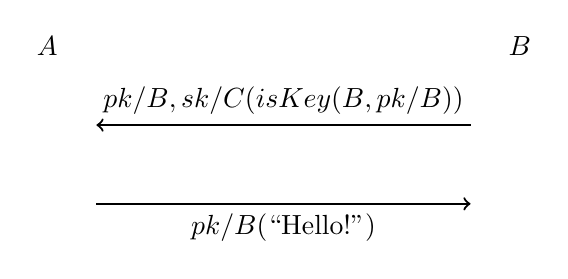
\begin{tikzpicture}
    \node at (-0.5,3) {$A$};
    \node at (5.5,3) {$B$};
    \node (a1) at (0,2) {};
    \node (b1) at (5,2) {};
    \draw[thick,->] (b1) -- (a1) node[above,midway]{${\mi{pk/B}, \sign{\mi{sk/C}}(\ms{isKey}(B, \mi{pk/B}))}$};
    \node (a2) at (0,1) {};
    \node (b2) at (5,1) {};
    \draw[thick,->] (a2) -- (b2) node[below,midway]{${\enc{\mi{pk/B}}(\mbox{``Hello!''})}$};
  \end{tikzpicture}
\]
Now suppose that a malicious party $M$ has obtained $C$'s secret
signing key. Then if $M$ is able to intercept all messages passed
between $A$ and $B$, they can read the encrypted messages intended for
$B$ as well as make changes to them. When $B$ sends $A$ its public key
and cert signed by $C$, then $M$ uses $C$'s signing key to certify a
chosen public key $\pk{B^\star}$ (with corresponding secret key
$\sk{B^\star}$ known to $M$), and forward $\pk{B^\star}$ to $A$ with
certification instead of $\pk{B}$. $A$ will believe that
$\pk{B^\star}$ is $B$'s public key because it came with a certificated
signed by trusted principal $C$, and use it to encrypt messages to $B$
as shown below.
\[
  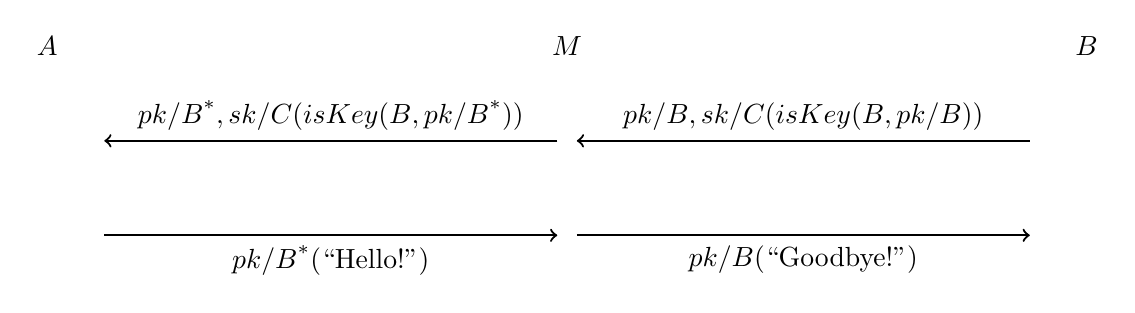
\begin{tikzpicture}[scale=1.2]
    \node at (-0.5,3) {$A$};
    \node at (5,3) {$M$};
    \node at (10.5,3) {$B$};
    \node (a1) at (0,2) {};
    \node (m1) at (5,2) {};
    \node (b1) at (10,2) {};
    \draw[thick,->] (b1) -- (m1) node[above,midway]{${\mi{pk/B}, \sign{\mi{sk/C}}(\ms{isKey}(B, \mi{pk/B}))}$};
    \draw[thick,->] (m1) -- (a1) node[above,midway]{${\mi{pk/B}^*, \sign{\mi{sk/C}}(\ms{isKey}(B, \mi{pk/B}^*))}$};
    \node (a2) at (0,1) {};
    \node (m2) at (5,1) {};
    \node (b2) at (10,1) {};
    \draw[thick,->] (a2) -- (m2) node[below,midway]{${\enc{\mi{pk/B}^*}(\mbox{``Hello!''})}$};
    \draw[thick,->] (m2) -- (b2) node[below,midway]{${\enc{\mi{pk/B}}(\mbox{``Goodbye!''})}$};
  \end{tikzpicture}
\]
Of course, because $M$ knows the corresponding secret key $\sk{B^\star}$, it can
decrypt and inspect the private messages $A$ sent to $B$. It can then choose to
either re-encrypt the original message with $\pk{B}$, or one of its
choosing. This is called a Man-in-the-Middle (MitM) attack, as the
attacker literally situates in between two parties who believe they are
communicating over a secure channel.

\section{Public key infrastructure}

So far we have glossed over the details of how certificate authorities
are assigned and managed. In the eduroam example, we assumed that
access points know the correct \pk{\mi{er}} because they are
provisioned expressly for the service, and come pre-loaded with the
necessary data. But certificates are used in all sorts of
applications, and it may not always be possible to transmit the CA's
key in such a way. How do principals come to trust a CA, and how does
the CA know that $\pk{A}$ actually belongs to $A$ in cases where it
does not generate the key? Answers to these questions entail defining
a Public Key Infrastructure (PKI), and there are several
alternatives for doing so.

\subsection{Centralized CA}

The most basic type of PKI consists of a single certificate authority
who is trusted by all principals to issue certificates for everyone's
public keys. Anyone who wants to use the PKI to establish trust in
other principals must obtain a secure copy of the CA's public keys,
and if they fail to accomplish this, then they will be unable to
verify legitimate certificates issued by the true CA, and may instead
end up ``verifying'' forged certificates issued by attackers.
Protecting against this possibility is typically accomplished by
obtaining a copy of the CA's key through physical contact, i.e.,
visiting the CA's offices and obtaining a file whose contents can be
compared against a known checksum. Likewise, to obtain a certificate
principals must usually present physical evidence of who they are, and
that the keys they wish to have signed actually belong to them.
Although the details of how this is done vary between CAs, the basic
process must be transparent and rigorous enough so that others trust
the CA's certs.

Another popular form of distribution for this model is to bundle
public keys for widely-known CAs with popular software. This is done
with browsers and operating systems, which typically implement a key
store that is pre-loaded with CA keys that can be automatically
verified as needed for validation. However, this approach is not
without its risks, as users are often tricked into downloading
corrupted versions of software that may have additional keys not
associated with real CAs pre-loaded into the store. In this event, all
of the failure modes discussed in the previous section are possible
and likely, which is why it is important to always verify checksums
for software that needs to interact with PKI.

This type of CA is usually a company that charges a fee to issue
certificates, or department within an organization tasked with
overseeing security. Because issuing certificates is a lucrative
business model, in practice there are many ``centralized'' CAs that
exist, and principals are free to choose whichever one they like when
purchasing certificates for their keys. In one important sense this
makes the overall PKI, in which users can choose which CAs to use and
trust, less brittle to compromise of any one CA's signing key. In
fact, it is considered good practice by some to obtain multiple
certificates for the same key, so that if one CA is corrupted then
others still have reason to trust the authenticity of the key.
However, most browsers and operating systems that come pre-loaded with
CA keys are configured to trust all of them equally, so really the
entire PKI is only as trustworthy as the least-trustworthy CA.
Ultimately, the responsibility is placed on end-users to configure
their settings in response to corrupt or compromised CAs as such
information becomes available. This is an unfortunate reality as most
users are not equipped to make such decisions, and fixing it remains
an open problem.

\subsection{Delegated trust and hierarchical CAs}

\begin{figure}
\centering
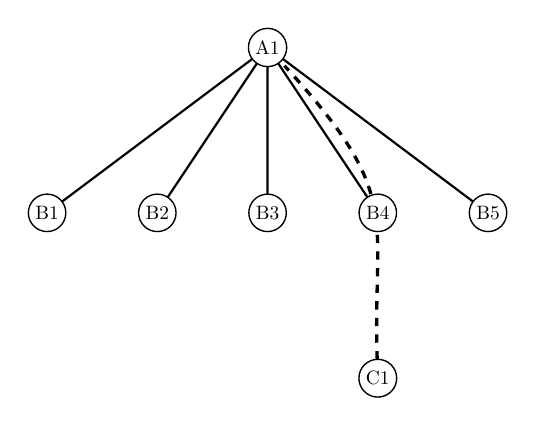
\begin{tikzpicture}[scale=0.7,transform shape]
  \Vertex[x=10,y=0]{A1}
  \Vertex[x=6,y=-3]{B1}
  \Vertex[x=8,y=-3]{B2}
  \Vertex[x=10,y=-3]{B3}
  \Vertex[x=12,y=-3]{B4}
  \Vertex[x=14,y=-3]{B5}
  \Vertex[x=12,y=-6]{C1}
  \tikzstyle{LabelStyle}=[fill=white]
  \Edge(A1)(B1)
  \Edge(A1)(B2)
  \Edge(A1)(B3)
  \Edge(A1)(B4)
  \Edge(A1)(B5)
  \path  (C1) .. controls (11.9,-3) and (12.5,-2.7) .. (A1)
     {\foreach \t [count=\i] in {0.00,0.01,...,0.99} {  coordinate[pos=\t] (p\i) } };
  \begin{pgfonlayer}{bg}
    \draw[dashed,very thick] (p1) { \foreach \i in {1,...,100} {-- (p\i) } };
  \end{pgfonlayer}
\end{tikzpicture}
\caption{\label{fig:ca-hierarchy}Hierarchical PKI model, where solid
lines correspond to existing trust relationships and the dashed curve to
the certificate chain that must be verified to build a new one. A1 is the root CA, and B1--B5 are
second-level subsidiary CAs. If
one wants to verify C1's certificate then they need to first check
that B4 signed C1's key, and then verify that A1 signed B4's key.}
\end{figure}

The reality of key compromise and the wide geographical reach of large
certificate authorities has led to the emergence of an alternative
hierarchical PKI. This model extends the centralized approach, and
still makes use of the key distribution and principal verification
strategies used by the centralized model. But now, the primary
``root'' CA delegates the ability to issue certificates to a
number of subsidiary or ``second-level'' CAs. Certificates issued by
second-level CAs then come with root-issued CAs themselves, thus
forming a ``certificate chain'' that can be verified in sequence until
reaching a trusted root CA with a known public key.

We can formalize this delegation policy using authorization logic. All that the
CA needs to do is sign propositions that denote which principals they trust to
sign on their behalf, e.g. with a predicate $\ms{trusts}(\ldots)$. Then the
subsidiary CA can attach the policy signed by the root CA to any certificate
that it issues using its delegation privilege.
\[
  \begin{array}{l}
    \mi{CA} \says (\forall x.\, \forall y.\, \forall \mi{pk}.\,
    \mi{CA} \says \ms{trusts}(x) \\
    \hspace{5em} \null \arrow x \says \ms{isKey}(y, \mi{pk}) \arrow \ms{isKey}(y, \mi{pk})
  \end{array}
\]
Checking that the rules described earlier allow others to make effective use of
subsidiary-issued certificates is left as an exercise.

An example of this model in action is shown in Figure~\ref{fig:ca-cert},
which is the current certificate provided when visiting
\nolinkurl{https://nytimes.com}. The root CA in this case is
COMODO RSA Certification Authority (we will call this $A$), and
the second-level CA is COMODO RSA Organization Validation Secure
Server CA (we will call this $B$), which is the principal who signed
the public key of \nolinkurl{nytimes.com}. The browser verifies that
the certificate for \nolinkurl{nytimes.com} was signed by $B$, and
that the certificate for $B$ was signed by the root CA $A$. In
addition, the browser will check that the root-signed certificate for
$B$'s public key is authorized to sign certificates itself; this is a
special ``extension'' field supported by the standard
(X.509~\citep{crl}) for digital certificates. This special
designation essentially says that $B$ is trusted by $A$ to issue
additional certificates on behalf of $A$, and that those certificates
should be treated as though they were issued by $A$ itself.

\begin{figure}
\centering
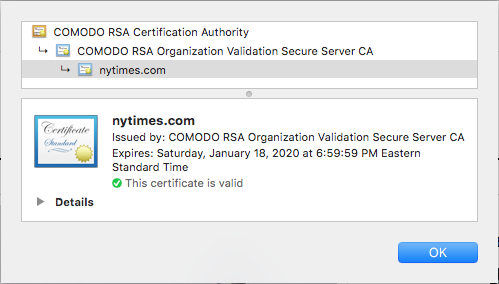
\includegraphics[width=0.7\textwidth]{19-trust-ca.png}
\caption{\label{fig:ca-cert}Example certificate chain used to authenticate
the secure \nolinkurl{nytimes.com} website, as displayed in the Chrome
browser.}
\end{figure}

The ability to delegate certification authority addresses many of the
practical hurdles in the centralized CA model. Certificate authorities
need to shoulder several burdens: ensuring the secrecy of the signing
key, ensuring that the public key is readily available for
verification, and vetting clients who wish to obtain certificates.
Splitting these responsibilities among several subsidiaries makes good
logistical sense. However, it also means that instead of just one
signing key, there are now several that must be kept secret. The root
CA must also ensure the integrity of subsidiary CAs, as they have the
ability to issue certificates on behalf of the root CA, and so the
trustworthiness of all related CAs is defined by the least trustworthy
subsidiary. In short, while the hierarchical model solves some
problems, it introduces several others.

Given that this model is in use on the Internet, exactly how many
different organizations can function as CAs and sign keys that your
web browser will trust?  A study done by the
\href{https://www.eff.org/observatory}{Electronic Frontier Foundation's
SSL Observatory} in 2010 found 651 distinct organizations functioning
as CAs.  Since then, the trend has been toward consolidation rather
than growth.  As of 2020, Mozilla's trust store contained 147 root
certificates from 52 organizations, and Google's Chrome Root Program
now enforces a limit of two root certificates per CA
owner~\citep{ChromeRootProgram}.  Stricter audit requirements and
compliance obligations have made it increasingly difficult for smaller
CAs to participate, concentrating issuance among a handful of large
organizations.

\paragraph{CA failures in practice.}
Two notable incidents illustrate the risks of this model.  In 2011,
the Dutch CA DigiNotar was completely compromised by an attacker who
gained administrative access to all of its signing
systems~\citep{DigiNotar11}.  The attacker issued over 500 fraudulent
certificates, including a wildcard certificate for \verb'google.com'
that was used to intercept the Gmail traffic of an estimated 300,000
Iranian users.  Because DigiNotar was a trusted CA in all major
browsers, every browser user in the world was potentially vulnerable
until the root was removed from trust stores.  DigiNotar was declared
bankrupt within a month.

A more protracted failure involved Symantec, which over several years
was found to have issued over 100 test certificates for domains it
did not control, including \verb'google.com' and
\verb'example.com'~\citep{SymantecDistrust}.  The initial mis-issuance
was discovered through Certificate Transparency logs.  Subsequent
investigation revealed broader compliance failures, and by 2018 all
major browsers had distrusted Symantec's root certificates.  Symantec
sold its certificate business to DigiCert.

These incidents illustrate a structural tension in the hierarchical
model.  Any trusted CA or subsidiary can issue a certificate for any
domain, and a single compromised or negligent CA can undermine the
security of the entire system.  In response, browser vendors now
actively police CAs, revoking trust from those that fail to meet
compliance standards.  This oversight, combined with Certificate
Transparency (discussed below), has significantly improved
accountability, but the underlying architectural tension remains.

\subsection{Automated certificate issuance: Let's Encrypt}

Traditionally, obtaining a certificate from a CA involved a manual process:
paying a fee, providing documentation of identity, and waiting for the CA to
verify and issue the certificate. This friction meant that many websites simply
did not use HTTPS, leaving their users vulnerable to eavesdropping and
man-in-the-middle attacks.

Let's Encrypt, launched in 2015 by the Internet Security Research Group (ISRG),
changed this by providing a free, automated CA. The central innovation is the
ACME (Automatic Certificate Management Environment) protocol, which allows a
server to obtain a certificate without any human intervention. The process works
as follows:
\begin{enumerate}
\item The server generates a public/secret key pair and sends a certificate
  request to Let's Encrypt.
\item Let's Encrypt issues a challenge to verify that the requester controls
  the domain. Typically, this involves placing a specific file at a known URL
  on the domain (HTTP challenge), or adding a specific DNS record (DNS
  challenge).
\item The server completes the challenge, Let's Encrypt verifies it, and issues
  a certificate binding the domain name to the server's public key.
\end{enumerate}

This is called domain validation (DV): the CA verifies only that the requester
controls the domain, not the identity of the organization behind it. This is a
weaker guarantee than organization validation (OV) or extended validation (EV)
certificates offered by traditional CAs, which require documentation of the
organization's legal identity. But for the vast majority of use cases,
where the goal is to ensure that traffic between a browser and a server
is encrypted and has not been tampered with, domain validation is sufficient.

Because the process is fully automated, Let's Encrypt issues certificates with
short lifetimes of 90 days, and clients are expected to renew them automatically
well before expiration. This stands in contrast to traditional CAs, which
typically issue certificates valid for one to two years. The short lifetime
limits the window of exposure if a key is compromised, and the automation means
that renewal imposes no burden on the server operator.

From the perspective of trust, Let's Encrypt operates within the same
hierarchical PKI that traditional CAs use. Its root certificate is included
in the trust stores of all major browsers and operating systems, so certificates
it issues are trusted by default. Initially, when Let's Encrypt's own root was
not yet widely trusted, its certificates were cross-signed by IdenTrust, an
established CA whose root was already in trust stores. This cross-signing
bootstrapped trust for Let's Encrypt using exactly the delegation mechanism
we formalized earlier.

Services similar to Let's Encrypt, such as ZeroSSL and Google Trust Services,
now also offer free automated certificates via ACME. The widespread adoption of
automated DV certificates has driven HTTPS adoption from roughly 40\% of web
page loads in 2015~\citep{Felt17usenix} to over 90\% today.

However, the DV model introduces its own failure modes. Because the only check
is domain control, an attacker who can temporarily hijack a domain's DNS records
or intercept its HTTP traffic can obtain a legitimate certificate for that
domain. BGP hijacking attacks, where an attacker reroutes traffic for a target's
IP prefix, have been used to pass ACME challenges and obtain fraudulent
certificates. Once the attacker has a valid certificate, they can mount a
man-in-the-middle attack that is indistinguishable from a legitimate connection.
Certificate Transparency logs (publicly auditable logs of all issued
certificates) provide a partial mitigation: domain owners can monitor these logs
and detect certificates they did not request, but this is a reactive rather than
preventive measure.

\subsection{Dealing with certificate compromise}

So far we have discussed the possible consequences of key compromise,
and weighed the potential ramifications of several PKI models on this
outcome. But what happens when a signing key becomes compromised? This
poses a significant challenge, as continued trust in signatures issued
with that key cripples the security of applications that rely on it.
The CA needs to disavow, or revoke, the compromised key
immediately while ensuring that users are aware that they should no
longer trust the old one. The PKI community has tried several
approaches over the years, and the landscape has shifted
significantly in recent years toward shorter certificate lifetimes and
public auditability.

\paragraph{Short-lived certificates.}
The most direct defense against key compromise is to issue certificates
with short lifetimes. Every certificate has an expiration date, as shown
in Figure~\ref{fig:ca-cert}, and once it passes, verifiers will no longer
trust the certificate. If certificates are short-lived enough, then a
compromised key is only useful for a brief window before the certificate
expires naturally, potentially eliminating the need for explicit
revocation altogether.

Traditionally, CA-issued certificates had lifetimes of one to several
years, because the manual process of obtaining and installing certificates
made frequent renewal impractical. As discussed above, automated CAs
like Let's Encrypt changed this calculus: automation makes 90-day lifetimes
routine, and Let's Encrypt has begun offering certificates valid for only
6 days. The CA/Browser Forum has been moving in this direction as well,
with a policy trajectory toward a maximum certificate lifetime of 47 days.

The appeal of short-lived certificates is that they sidestep the revocation
problem entirely. If a certificate is only valid for a week, then by the
time anyone discovers a key compromise and mobilizes a response, the
certificate is likely already expired. The tradeoff is that the
infrastructure must support fully automated renewal, and any failure in
the renewal pipeline (e.g., a misconfigured server or an expired domain)
results in an outage.

\paragraph{Certificate revocation lists.}
When certificates have longer lifetimes, explicit revocation is necessary.
The standard mechanism is for the CA to maintain a certificate revocation
list (CRL)~\citep{crl}. Each certificate is given a unique serial number,
and if the key becomes compromised, the CA adds that serial number to
the CRL. Verifiers are responsible for obtaining and cross-referencing
the current CRL when checking a certificate.

In 2024, the CA/Browser Forum made CRLs mandatory for all CAs, reflecting
their status as the baseline revocation mechanism. CRLs can grow large
and must be fetched regularly, and if the CRL server goes offline then
verifiers cannot check revocation status. On the other hand, they are
simple, well-understood, and do not leak information about which sites
a user visits.

An alternative called OCSP (Online Certificate Status Protocol) allowed
verifiers to query the CA about individual certificates on demand rather
than downloading full lists~\citep{ocsp}. While this reduced bandwidth,
OCSP raised serious privacy concerns: each query told the CA (and anyone
eavesdropping on the unencrypted OCSP traffic) which website the user was
visiting. In practice, most browsers silently ignored OCSP failures rather
than blocking access, which meant OCSP provided little actual security
benefit. Let's Encrypt shut down its OCSP responders entirely in 2025,
and the industry has largely moved away from the protocol.

\paragraph{Certificate Transparency.}
A complementary approach to revocation is Certificate Transparency (CT),
which addresses a different question: how do we detect certificates that
should never have been issued in the first place? CT requires CAs to
submit every certificate they issue to one or more publicly auditable,
append-only logs. Domain owners, browser vendors, and researchers can
all monitor these logs and detect suspicious certificates, such as a
certificate for \verb'cmu.edu' issued by a CA that CMU has never used.

CT does not prevent mis-issuance, but it makes it visible. This is a reactive
rather than preventive measure, but it has proven effective in practice.
Several high-profile incidents of CA misbehavior were discovered through
CT logs, and all major browsers now require CT compliance for certificates
to be trusted. Concretely, this is enforced during the TLS handshake: the
browser checks that the certificate is accompanied by Signed Certificate
Timestamps (SCTs), which are cryptographic proofs from log operators that
the certificate has been recorded. If the SCTs are missing or insufficient,
the browser rejects the connection outright.  Domain owners can set up
automated monitoring to be alerted whenever a new certificate is issued for
their domain, allowing them to respond quickly to unauthorized certificates.

An earlier approach called HTTP Public Key Pinning (HPKP) attempted to
solve the same problem proactively: domain owners could specify which CAs
were authorized to issue certificates for their domain, and browsers would
reject certificates from other CAs. However, HPKP was deprecated by
browsers in 2018 because misconfiguration could permanently lock
legitimate owners out of their own domains. CT monitoring, combined with
DNS Certification Authority Authorization (CAA) records that instruct CAs
not to issue unauthorized certificates, has largely replaced pinning as
the standard defense against CA compromise.

\section{Practice Problems}

These problems are for self-study and are not to be handed in.

\subsection{Certificate Chains [3 parts]}

Suppose a browser trusts root CA $\mi{rootCA}$ and has its public key
$\pk{\mi{rootCA}}$.  A user visits \verb'shop.example.com', and the server
presents:
\begin{enumerate}[(i)]
\item A certificate $\cert{\mi{rootCA}}{\mi{subCA}}(\pk{\mi{subCA}})$
\item A certificate $\cert{\mi{subCA}}{\mi{shop}}(\pk{\mi{shop}})$
\item A signature $\sign{\sk{\mi{shop}}}(\ms{isServer}(\mi{shop.example.com}))$
\end{enumerate}

\begin{task}\rm
  Using the $\mb{says}/\mb{sign}$ and $\mb{cert}$ rules from the lecture,
  write out a proof term that establishes
  $\mi{subCA} \says \ms{isKey}(\mi{shop}, \pk{\mi{shop}})$
  from the certificates above, assuming $\ms{isCA}(\mi{rootCA})$ and
  $\ms{isKey}(\mi{rootCA}, \pk{\mi{rootCA}})$.
\end{task}

\begin{task}\rm
  Now suppose $\mi{subCA}$'s secret key is compromised.  An attacker
  generates a fresh key pair $\langle \pk{\star}, \sk{\star} \rangle$
  and produces $\cert{\mi{subCA}}{\mi{shop}}(\pk{\star})$.  Describe
  the messages the attacker would send to mount a man-in-the-middle
  attack against a user connecting to \verb'shop.example.com'.
\end{task}

\begin{task}\rm
  Which of the following defenses would detect or prevent the attack
  from the previous task?  Briefly justify each answer.
  \begin{enumerate}
  \item Certificate Transparency logs
  \item Certificate revocation lists
  \item Short-lived certificates (e.g., 6-day lifetime)
  \item DNS CAA records
  \end{enumerate}
\end{task}

\subsection{Domain Validation and Trust [3 parts]}

Recall that Let's Encrypt uses domain validation: the CA issues a
challenge (e.g., ``place this file at
\verb'http://example.com/.well-known/acme-challenge/TOKEN'\,''),
and issues a certificate if the challenge is completed.

An attacker performs a BGP hijacking attack, temporarily rerouting
traffic destined for $\mi{example.com}$'s IP address to a server
under the attacker's control.  The attacker completes the ACME
challenge and obtains a valid certificate for $\mi{example.com}$.
After the BGP hijack ends, the attacker uses this certificate to
impersonate $\mi{example.com}$ from a different network location.

\begin{task}\rm
  Write out the message sequence (public key, certificates, signatures)
  that the attacker's server would present to a connecting browser.
  For each message, state which principal's key was used and whether
  the message is legitimate or fraudulent.
\end{task}

\begin{task}\rm
  Using the $\mb{says}/\mb{sign}$ and $\mb{cert}$ rules, write out a
  proof sketch showing why the browser accepts this message sequence.
  At which step in the proof does the fraudulent assumption enter, and
  why can the browser not detect it?
\end{task}

\begin{task}\rm
  The owner of $\mi{example.com}$ requests revocation of the
  unauthorized certificate.  Suppose the certificate was issued with
  a 90-day lifetime and the owner detects it via CT logs 12 hours
  after issuance.  For each of the following, state whether the
  unauthorized certificate would still be accepted by a browser
  connecting 24 hours after issuance.
  \begin{enumerate}
  \item The CA publishes an updated CRL within 6 hours of the
    revocation request, and the browser checks the CRL.
  \item The CA publishes an updated CRL within 6 hours, but the
    browser fails to reach the CRL server and uses soft-fail.
  \item The certificate had been issued with a 6-day lifetime instead
    of 90 days.
  \end{enumerate}
\end{task}

\bibliographystyle{plainnat}
\bibliography{bibliography}

\end{document}
